\documentclass[11pt]{article}
\usepackage{subcaption}
\usepackage{sectsty}
\usepackage{graphicx}
\usepackage{amsmath} % for 'pmatrix' environment
\usepackage{caption}
\usepackage{subcaption}

% Margins
\topmargin=-0.45in
\evensidemargin=0in
\oddsidemargin=0in
\textwidth=6.5in
\textheight=9.0in
\headsep=0.25in

\title{\textbf{Dokumentation zu:\\DRL-Aufgabenblatt "Markov Decision Processes"}}
\author{Erik Viere, Daniel Hilfer, Domenic Scholz}
\date{\today}

\begin{document}
\maketitle	
\pagebreak

\section*{Aufgabe 3.1}
\subsection*{a)}
Der Algorithmus ist im zugehörigen Jupyter-Notebook dargestellt. Auch die Visualisierungen lassen sich dort finden. Zur Vollständigkeit werden die finalen State Values sowie die finale Policy auch noch einmal in Abbildung  \ref{img:3_1_a} dargestellt. Eine Erklärung der jeweiligen Zeichen ist ebenfalls als Code-Kommentar im Jupyter-Notebook zu finden.\\
Die Konvergenz der State Values tritt in diesem Fall ein, wenn sich kein Wert in der aktuellen Iteration um mehr als $0.001$ geändert hat. Dies dauert $30$ Iterationen für den ersten Durchlauf. Nach diesem wurde die Policy aktualisiert. Der zweite Durchlauf, der bestätigt hat, dass es sich bei der aktualisierten Policy um die beste handelt, brauchte $28$ Iterationen bis zur Konvergenz.

\begin{figure}
    \centering
    \begin{subfigure}[t]{0.32\textwidth}
        \centering
        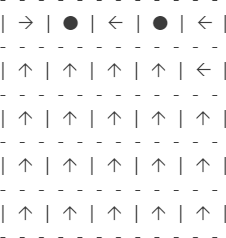
\includegraphics[width=\textwidth]{img/3_1_a1.png}
        \caption{Finale Policy mithilfe bereits konvergierter State Values}
        \label{img:3_1_a1}
    \end{subfigure}
    \hfill
    \begin{subfigure}[t]{0.65\textwidth}
        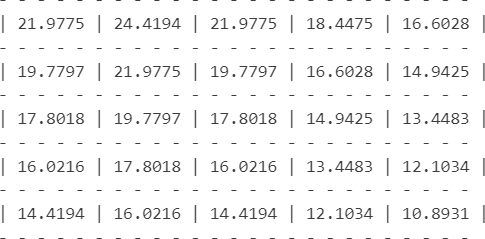
\includegraphics[width=\textwidth]{img/3_1_a2.png}
        \caption{Finale State Values nach Anwendung der optimalen Policy}
        \label{img:3_1_a2}
    \end{subfigure}
    \caption{Ergebnisse des GPI Algorithmus mit vollständer State Value Konvergenz}
    \label{img:3_1_a}
\end{figure}

\subsection*{b)}
Die Implementierung des Algorithmus ist auch für diesen Aufgabenteil im Jupyter-Notebook zu finden.

\subsection*{c)}
\end{document}